\section{Spark::Sp\-Turbulence\-Op Class Reference}
\label{classSpark_1_1SpTurbulenceOp}\index{Spark::SpTurbulenceOp@{Spark::SpTurbulenceOp}}
{\tt \#include $<$Sp\-Turbulence\-Op.h$>$}

Inheritance diagram for Spark::Sp\-Turbulence\-Op:\begin{figure}[H]
\begin{center}
\leavevmode
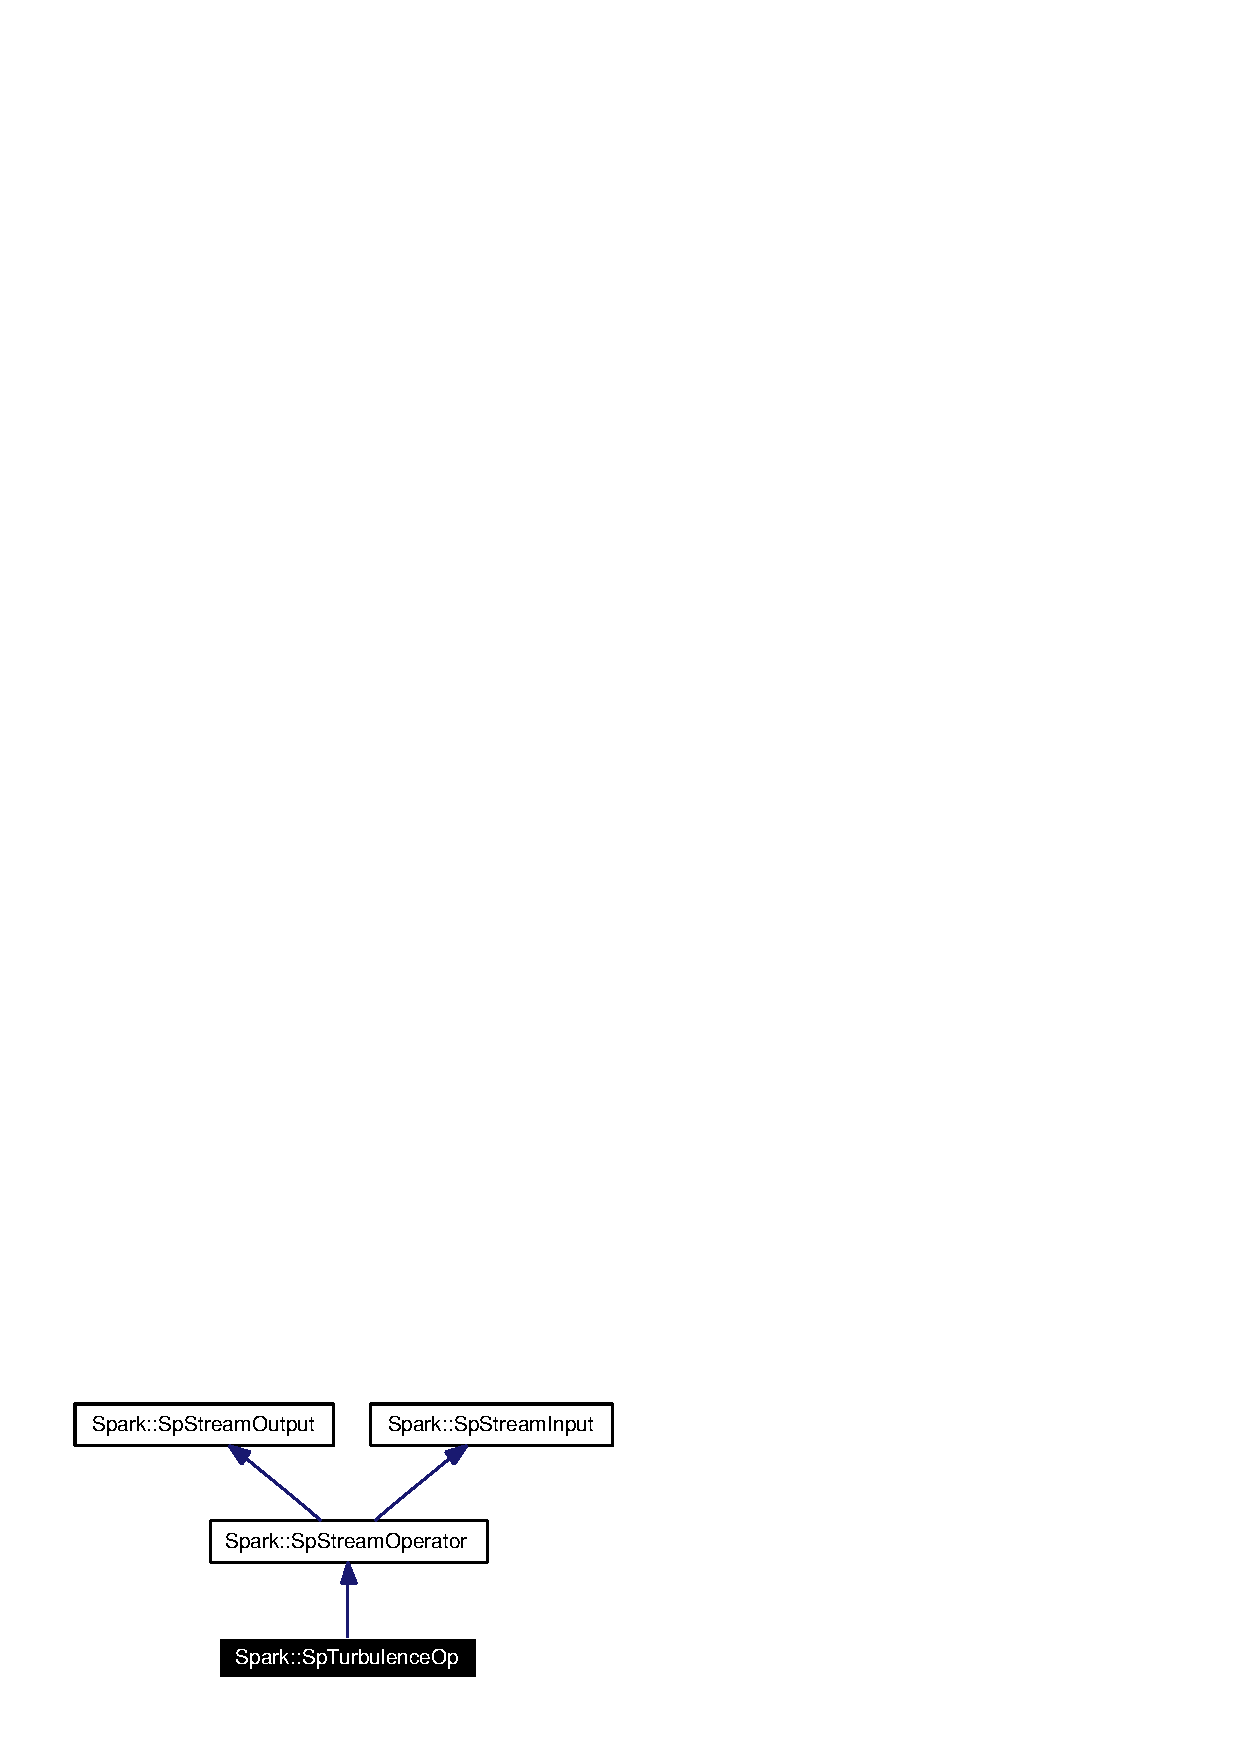
\includegraphics[width=147pt]{classSpark_1_1SpTurbulenceOp__inherit__graph}
\end{center}
\end{figure}
Collaboration diagram for Spark::Sp\-Turbulence\-Op:\begin{figure}[H]
\begin{center}
\leavevmode
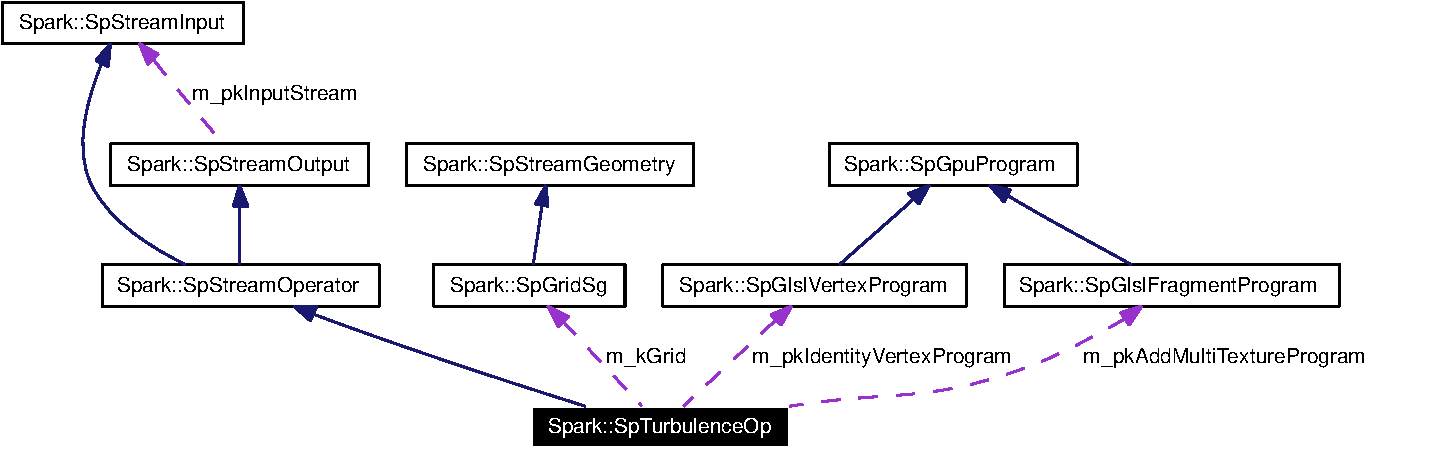
\includegraphics[width=362pt]{classSpark_1_1SpTurbulenceOp__coll__graph}
\end{center}
\end{figure}


\subsection{Detailed Description}
Turbulence stream operator to be used with a stream basis class. 

Definition at line 39 of file Sp\-Turbulence\-Op.h.\subsection*{Public Member Functions}
\begin{CompactItemize}
\item 
{\bf Sp\-Turbulence\-Op} (float f\-X=1, float f\-Y=1, float f\-Z=1, float f\-Octaves=4, float f\-Increment=0.5f, float f\-Lacunarity=2.0345f)
\begin{CompactList}\small\item\em Construction:. \item\end{CompactList}\item 
virtual {\bf $\sim$Sp\-Turbulence\-Op} ()
\item 
void {\bf initialize} ({\bf Sp\-Stream\-Buffer} $\ast$pk\-Buffer, {\bf Sp\-Stream\-Feedback} $\ast$pk\-Copy, bool b\-Create\-Textures)
\item 
virtual void {\bf set\-Input\-Stream} ({\bf Sp\-Stream\-Basis} $\ast$pk\-Input\-Stream)
\begin{CompactList}\small\item\em Access Methods:. \item\end{CompactList}\item 
virtual void {\bf set\-Input\-Stream} ({\bf Sp\-Stream\-Input} $\ast$pk\-Input\-Stream)
\begin{CompactList}\small\item\em Operations:. \item\end{CompactList}\item 
void {\bf set\-Octaves} (float f\-Octaves)
\item 
float {\bf get\-Octaves} () const
\item 
void {\bf set\-Lacunarity} (float f\-Lacunarity)
\item 
float {\bf get\-Lacunarity} () const
\item 
void {\bf set\-Increment} (float f\-Increment)
\item 
float {\bf get\-Increment} () const
\item 
virtual void {\bf set\-Offset} (float f\-X, float f\-Y, float f\-Z)
\item 
virtual void {\bf get\-Offset} (float \&rf\-X, float \&rf\-Y, float \&rf\-Z) const
\end{CompactItemize}
\subsection*{Protected Member Functions}
\begin{CompactItemize}
\item 
virtual bool {\bf enable\-Output\-Stream} ({\bf Sp\-Stream\-Buffer} $\ast$pk\-Buffer, {\bf Sp\-Stream\-Feedback} $\ast$pk\-Copy)
\begin{CompactList}\small\item\em Internal Methods:. \item\end{CompactList}\item 
virtual bool {\bf setup\-State} ({\bf Sp\-Stream\-Buffer} $\ast$pk\-Buffer, {\bf Sp\-Stream\-Feedback} $\ast$pk\-Copy)
\item 
virtual bool {\bf process\-Stream} ({\bf Sp\-Stream\-Buffer} $\ast$pk\-Buffer, {\bf Sp\-Stream\-Feedback} $\ast$pk\-Copy)
\item 
virtual bool {\bf update\-Output\-Stream} ({\bf Sp\-Stream\-Buffer} $\ast$pk\-Buffer, {\bf Sp\-Stream\-Feedback} $\ast$pk\-Copy)
\item 
virtual bool {\bf reset\-State} ({\bf Sp\-Stream\-Buffer} $\ast$pk\-Buffer, {\bf Sp\-Stream\-Feedback} $\ast$pk\-Copy)
\item 
virtual bool {\bf disable\-Output\-Stream} ({\bf Sp\-Stream\-Buffer} $\ast$pk\-Buffer, {\bf Sp\-Stream\-Feedback} $\ast$pk\-Copy)
\end{CompactItemize}
\subsection*{Protected Attributes}
\begin{CompactItemize}
\item 
float {\bf m\_\-f\-Octaves}
\begin{CompactList}\small\item\em Internal Data:. \item\end{CompactList}\item 
float {\bf m\_\-f\-Lacunarity}
\item 
float {\bf m\_\-f\-Increment}
\item 
float {\bf m\_\-f\-Offset\-X}
\item 
float {\bf m\_\-f\-Offset\-Y}
\item 
float {\bf m\_\-f\-Offset\-Z}
\item 
float {\bf m\_\-f\-X}
\item 
float {\bf m\_\-f\-Y}
\item 
float {\bf m\_\-f\-Z}
\item 
unsigned int {\bf m\_\-ui\-Current\-Pass}
\item 
unsigned int {\bf m\_\-ui\-Max\-Octaves}
\item 
bool {\bf m\_\-b\-Input\-Is\-Basis}
\item 
bool {\bf m\_\-b\-Create\-Textures}
\item 
bool {\bf m\_\-b\-Initialized}
\item 
double $\ast$ {\bf m\_\-ad\-Exponents}
\item 
{\bf Sp\-Grid\-Sg} {\bf m\_\-k\-Grid}
\item 
unsigned int $\ast$ {\bf m\_\-aui\-Textures}
\item 
unsigned int {\bf m\_\-ui\-Texture\-Count}
\item 
{\bf Sp\-Glsl\-Vertex\-Program} $\ast$ {\bf m\_\-pk\-Identity\-Vertex\-Program}
\item 
{\bf Sp\-Glsl\-Fragment\-Program} $\ast$ {\bf m\_\-pk\-Add\-Multi\-Texture\-Program}
\end{CompactItemize}


\subsection{Constructor \& Destructor Documentation}
\index{Spark::SpTurbulenceOp@{Spark::Sp\-Turbulence\-Op}!SpTurbulenceOp@{SpTurbulenceOp}}
\index{SpTurbulenceOp@{SpTurbulenceOp}!Spark::SpTurbulenceOp@{Spark::Sp\-Turbulence\-Op}}
\subsubsection{\setlength{\rightskip}{0pt plus 5cm}Sp\-Turbulence\-Op::Sp\-Turbulence\-Op (float {\em f\-X} = {\tt 1}, float {\em f\-Y} = {\tt 1}, float {\em f\-Z} = {\tt 1}, float {\em f\-Octaves} = {\tt 4}, float {\em f\-Increment} = {\tt 0.5f}, float {\em f\-Lacunarity} = {\tt 2.0345f})}\label{classSpark_1_1SpTurbulenceOp_a0}


Construction:. 

Definition at line 27 of file Sp\-Turbulence\-Op.cpp.

References m\_\-ad\-Exponents, m\_\-aui\-Textures, m\_\-f\-Octaves, m\_\-ui\-Max\-Octaves, and m\_\-ui\-Texture\-Count.\index{Spark::SpTurbulenceOp@{Spark::Sp\-Turbulence\-Op}!~SpTurbulenceOp@{$\sim$SpTurbulenceOp}}
\index{~SpTurbulenceOp@{$\sim$SpTurbulenceOp}!Spark::SpTurbulenceOp@{Spark::Sp\-Turbulence\-Op}}
\subsubsection{\setlength{\rightskip}{0pt plus 5cm}Sp\-Turbulence\-Op::$\sim${\bf Sp\-Turbulence\-Op} ()\hspace{0.3cm}{\tt  [virtual]}}\label{classSpark_1_1SpTurbulenceOp_a1}


Definition at line 94 of file Sp\-Turbulence\-Op.cpp.

References Spark::Sp\-Gl\-Manager::delete\-Texture(), m\_\-ad\-Exponents, m\_\-aui\-Textures, and m\_\-ui\-Texture\-Count.

\subsection{Member Function Documentation}
\index{Spark::SpTurbulenceOp@{Spark::Sp\-Turbulence\-Op}!disableOutputStream@{disableOutputStream}}
\index{disableOutputStream@{disableOutputStream}!Spark::SpTurbulenceOp@{Spark::Sp\-Turbulence\-Op}}
\subsubsection{\setlength{\rightskip}{0pt plus 5cm}bool Sp\-Turbulence\-Op::disable\-Output\-Stream ({\bf Sp\-Stream\-Buffer} $\ast$ {\em pk\-Buffer}, {\bf Sp\-Stream\-Feedback} $\ast$ {\em pk\-Copy})\hspace{0.3cm}{\tt  [protected, virtual]}}\label{classSpark_1_1SpTurbulenceOp_b5}




Reimplemented from {\bf Spark::Sp\-Stream\-Operator} {\rm (p.\,\pageref{classSpark_1_1SpStreamOperator_b6})}.

Definition at line 312 of file Sp\-Turbulence\-Op.cpp.\index{Spark::SpTurbulenceOp@{Spark::Sp\-Turbulence\-Op}!enableOutputStream@{enableOutputStream}}
\index{enableOutputStream@{enableOutputStream}!Spark::SpTurbulenceOp@{Spark::Sp\-Turbulence\-Op}}
\subsubsection{\setlength{\rightskip}{0pt plus 5cm}bool Sp\-Turbulence\-Op::enable\-Output\-Stream ({\bf Sp\-Stream\-Buffer} $\ast$ {\em pk\-Buffer}, {\bf Sp\-Stream\-Feedback} $\ast$ {\em pk\-Copy})\hspace{0.3cm}{\tt  [protected, virtual]}}\label{classSpark_1_1SpTurbulenceOp_b0}


Internal Methods:. 



Reimplemented from {\bf Spark::Sp\-Stream\-Operator} {\rm (p.\,\pageref{classSpark_1_1SpStreamOperator_b1})}.

Definition at line 183 of file Sp\-Turbulence\-Op.cpp.

References Spark::Sp\-Stream\-Buffer::get\-Height(), Spark::Sp\-Stream\-Buffer::get\-Texture\-Target(), Spark::Sp\-Stream\-Buffer::get\-Width(), m\_\-aui\-Textures, m\_\-f\-Octaves, m\_\-ui\-Current\-Pass, and Spark::Sp\-Stream\-Feedback::set\-Output\-Texture().\index{Spark::SpTurbulenceOp@{Spark::Sp\-Turbulence\-Op}!getIncrement@{getIncrement}}
\index{getIncrement@{getIncrement}!Spark::SpTurbulenceOp@{Spark::Sp\-Turbulence\-Op}}
\subsubsection{\setlength{\rightskip}{0pt plus 5cm}float Sp\-Turbulence\-Op::get\-Increment () const}\label{classSpark_1_1SpTurbulenceOp_a10}


Definition at line 344 of file Sp\-Turbulence\-Op.cpp.

References m\_\-f\-Increment.\index{Spark::SpTurbulenceOp@{Spark::Sp\-Turbulence\-Op}!getLacunarity@{getLacunarity}}
\index{getLacunarity@{getLacunarity}!Spark::SpTurbulenceOp@{Spark::Sp\-Turbulence\-Op}}
\subsubsection{\setlength{\rightskip}{0pt plus 5cm}float Sp\-Turbulence\-Op::get\-Lacunarity () const}\label{classSpark_1_1SpTurbulenceOp_a8}


Definition at line 328 of file Sp\-Turbulence\-Op.cpp.

References m\_\-f\-Lacunarity.\index{Spark::SpTurbulenceOp@{Spark::Sp\-Turbulence\-Op}!getOctaves@{getOctaves}}
\index{getOctaves@{getOctaves}!Spark::SpTurbulenceOp@{Spark::Sp\-Turbulence\-Op}}
\subsubsection{\setlength{\rightskip}{0pt plus 5cm}float Sp\-Turbulence\-Op::get\-Octaves () const}\label{classSpark_1_1SpTurbulenceOp_a6}


Definition at line 379 of file Sp\-Turbulence\-Op.cpp.

References m\_\-f\-Octaves.\index{Spark::SpTurbulenceOp@{Spark::Sp\-Turbulence\-Op}!getOffset@{getOffset}}
\index{getOffset@{getOffset}!Spark::SpTurbulenceOp@{Spark::Sp\-Turbulence\-Op}}
\subsubsection{\setlength{\rightskip}{0pt plus 5cm}void Sp\-Turbulence\-Op::get\-Offset (float \& {\em rf\-X}, float \& {\em rf\-Y}, float \& {\em rf\-Z}) const\hspace{0.3cm}{\tt  [virtual]}}\label{classSpark_1_1SpTurbulenceOp_a12}


Definition at line 358 of file Sp\-Turbulence\-Op.cpp.

References m\_\-f\-Offset\-X, m\_\-f\-Offset\-Y, and m\_\-f\-Offset\-Z.\index{Spark::SpTurbulenceOp@{Spark::Sp\-Turbulence\-Op}!initialize@{initialize}}
\index{initialize@{initialize}!Spark::SpTurbulenceOp@{Spark::Sp\-Turbulence\-Op}}
\subsubsection{\setlength{\rightskip}{0pt plus 5cm}void Sp\-Turbulence\-Op::initialize ({\bf Sp\-Stream\-Buffer} $\ast$ {\em pk\-Buffer}, {\bf Sp\-Stream\-Feedback} $\ast$ {\em pk\-Copy}, bool {\em b\-Create\-Textures})}\label{classSpark_1_1SpTurbulenceOp_a2}


Definition at line 103 of file Sp\-Turbulence\-Op.cpp.

References Spark::Sp\-Glsl\-Manager::compile(), Spark::Sp\-Gl\-Manager::create\-Filtered\-Texture(), Spark::Sp\-Gl\-Manager::delete\-Texture(), Spark::Sp\-Stream\-Buffer::get\-Height(), Spark::Sp\-Stream\-Buffer::get\-Texture\-Target(), Spark::Sp\-Stream\-Buffer::get\-Width(), Spark::Sp\-Stream\-Buffer::is\-Rectangle\-Texture(), Spark::Sp\-Glsl\-Manager::load\-Fragment\-Program\-From\-File(), Spark::Sp\-Glsl\-Manager::load\-Vertex\-Program\-From\-File(), m\_\-ad\-Exponents, m\_\-aui\-Textures, m\_\-b\-Create\-Textures, m\_\-b\-Initialized, m\_\-f\-Increment, m\_\-f\-Lacunarity, m\_\-pk\-Add\-Multi\-Texture\-Program, m\_\-pk\-Identity\-Vertex\-Program, m\_\-ui\-Current\-Pass, m\_\-ui\-Max\-Octaves, m\_\-ui\-Texture\-Count, and Spark::Pow().

Referenced by setup\-State().\index{Spark::SpTurbulenceOp@{Spark::Sp\-Turbulence\-Op}!processStream@{processStream}}
\index{processStream@{processStream}!Spark::SpTurbulenceOp@{Spark::Sp\-Turbulence\-Op}}
\subsubsection{\setlength{\rightskip}{0pt plus 5cm}bool Sp\-Turbulence\-Op::process\-Stream ({\bf Sp\-Stream\-Buffer} $\ast$ {\em pk\-Buffer}, {\bf Sp\-Stream\-Feedback} $\ast$ {\em pk\-Copy})\hspace{0.3cm}{\tt  [protected, virtual]}}\label{classSpark_1_1SpTurbulenceOp_b2}




Reimplemented from {\bf Spark::Sp\-Stream\-Operator} {\rm (p.\,\pageref{classSpark_1_1SpStreamOperator_b3})}.

Definition at line 223 of file Sp\-Turbulence\-Op.cpp.

References m\_\-f\-Octaves, m\_\-ui\-Current\-Pass, and Spark::Sp\-Stream\-Input::send\-Output\-To\-Buffer().\index{Spark::SpTurbulenceOp@{Spark::Sp\-Turbulence\-Op}!resetState@{resetState}}
\index{resetState@{resetState}!Spark::SpTurbulenceOp@{Spark::Sp\-Turbulence\-Op}}
\subsubsection{\setlength{\rightskip}{0pt plus 5cm}bool Sp\-Turbulence\-Op::reset\-State ({\bf Sp\-Stream\-Buffer} $\ast$ {\em pk\-Buffer}, {\bf Sp\-Stream\-Feedback} $\ast$ {\em pk\-Copy})\hspace{0.3cm}{\tt  [protected, virtual]}}\label{classSpark_1_1SpTurbulenceOp_b4}




Reimplemented from {\bf Spark::Sp\-Stream\-Operator} {\rm (p.\,\pageref{classSpark_1_1SpStreamOperator_b5})}.

Definition at line 286 of file Sp\-Turbulence\-Op.cpp.

References m\_\-f\-Lacunarity, m\_\-f\-Octaves, m\_\-f\-Offset\-X, m\_\-f\-Offset\-Y, m\_\-f\-Offset\-Z, m\_\-f\-X, m\_\-f\-Y, m\_\-f\-Z, and m\_\-ui\-Current\-Pass.\index{Spark::SpTurbulenceOp@{Spark::Sp\-Turbulence\-Op}!setIncrement@{setIncrement}}
\index{setIncrement@{setIncrement}!Spark::SpTurbulenceOp@{Spark::Sp\-Turbulence\-Op}}
\subsubsection{\setlength{\rightskip}{0pt plus 5cm}void Sp\-Turbulence\-Op::set\-Increment (float {\em f\-Increment})}\label{classSpark_1_1SpTurbulenceOp_a9}


Definition at line 334 of file Sp\-Turbulence\-Op.cpp.

References m\_\-b\-Initialized, and m\_\-f\-Increment.\index{Spark::SpTurbulenceOp@{Spark::Sp\-Turbulence\-Op}!setInputStream@{setInputStream}}
\index{setInputStream@{setInputStream}!Spark::SpTurbulenceOp@{Spark::Sp\-Turbulence\-Op}}
\subsubsection{\setlength{\rightskip}{0pt plus 5cm}void Sp\-Turbulence\-Op::set\-Input\-Stream ({\bf Sp\-Stream\-Input} $\ast$ {\em pk\-Input\-Stream})\hspace{0.3cm}{\tt  [virtual]}}\label{classSpark_1_1SpTurbulenceOp_a4}


Operations:. 



Reimplemented from {\bf Spark::Sp\-Stream\-Operator} {\rm (p.\,\pageref{classSpark_1_1SpStreamOperator_a2})}.

Definition at line 390 of file Sp\-Turbulence\-Op.cpp.

References m\_\-b\-Input\-Is\-Basis, and Spark::Sp\-Stream\-Operator::set\-Input\-Stream().\index{Spark::SpTurbulenceOp@{Spark::Sp\-Turbulence\-Op}!setInputStream@{setInputStream}}
\index{setInputStream@{setInputStream}!Spark::SpTurbulenceOp@{Spark::Sp\-Turbulence\-Op}}
\subsubsection{\setlength{\rightskip}{0pt plus 5cm}void Sp\-Turbulence\-Op::set\-Input\-Stream ({\bf Sp\-Stream\-Basis} $\ast$ {\em pk\-Input\-Stream})\hspace{0.3cm}{\tt  [virtual]}}\label{classSpark_1_1SpTurbulenceOp_a3}


Access Methods:. 

Definition at line 384 of file Sp\-Turbulence\-Op.cpp.

References m\_\-b\-Input\-Is\-Basis, and Spark::Sp\-Stream\-Operator::set\-Input\-Stream().\index{Spark::SpTurbulenceOp@{Spark::Sp\-Turbulence\-Op}!setLacunarity@{setLacunarity}}
\index{setLacunarity@{setLacunarity}!Spark::SpTurbulenceOp@{Spark::Sp\-Turbulence\-Op}}
\subsubsection{\setlength{\rightskip}{0pt plus 5cm}void Sp\-Turbulence\-Op::set\-Lacunarity (float {\em f\-Lacunarity})}\label{classSpark_1_1SpTurbulenceOp_a7}


Definition at line 318 of file Sp\-Turbulence\-Op.cpp.

References m\_\-b\-Initialized, and m\_\-f\-Lacunarity.\index{Spark::SpTurbulenceOp@{Spark::Sp\-Turbulence\-Op}!setOctaves@{setOctaves}}
\index{setOctaves@{setOctaves}!Spark::SpTurbulenceOp@{Spark::Sp\-Turbulence\-Op}}
\subsubsection{\setlength{\rightskip}{0pt plus 5cm}void Sp\-Turbulence\-Op::set\-Octaves (float {\em f\-Octaves})}\label{classSpark_1_1SpTurbulenceOp_a5}


Definition at line 365 of file Sp\-Turbulence\-Op.cpp.

References m\_\-b\-Create\-Textures, m\_\-b\-Initialized, m\_\-f\-Octaves, and m\_\-ui\-Max\-Octaves.\index{Spark::SpTurbulenceOp@{Spark::Sp\-Turbulence\-Op}!setOffset@{setOffset}}
\index{setOffset@{setOffset}!Spark::SpTurbulenceOp@{Spark::Sp\-Turbulence\-Op}}
\subsubsection{\setlength{\rightskip}{0pt plus 5cm}void Sp\-Turbulence\-Op::set\-Offset (float {\em f\-X}, float {\em f\-Y}, float {\em f\-Z})\hspace{0.3cm}{\tt  [virtual]}}\label{classSpark_1_1SpTurbulenceOp_a11}


Definition at line 349 of file Sp\-Turbulence\-Op.cpp.

References m\_\-f\-Offset\-X, m\_\-f\-Offset\-Y, m\_\-f\-Offset\-Z, and m\_\-ui\-Current\-Pass.\index{Spark::SpTurbulenceOp@{Spark::Sp\-Turbulence\-Op}!setupState@{setupState}}
\index{setupState@{setupState}!Spark::SpTurbulenceOp@{Spark::Sp\-Turbulence\-Op}}
\subsubsection{\setlength{\rightskip}{0pt plus 5cm}bool Sp\-Turbulence\-Op::setup\-State ({\bf Sp\-Stream\-Buffer} $\ast$ {\em pk\-Buffer}, {\bf Sp\-Stream\-Feedback} $\ast$ {\em pk\-Copy})\hspace{0.3cm}{\tt  [protected, virtual]}}\label{classSpark_1_1SpTurbulenceOp_b1}




Reimplemented from {\bf Spark::Sp\-Stream\-Operator} {\rm (p.\,\pageref{classSpark_1_1SpStreamOperator_b2})}.

Definition at line 199 of file Sp\-Turbulence\-Op.cpp.

References initialize(), m\_\-ad\-Exponents, m\_\-b\-Create\-Textures, m\_\-b\-Initialized, m\_\-b\-Input\-Is\-Basis, m\_\-f\-Octaves, m\_\-f\-Offset\-X, m\_\-f\-Offset\-Y, m\_\-f\-Offset\-Z, m\_\-f\-X, m\_\-f\-Y, m\_\-f\-Z, m\_\-ui\-Current\-Pass, Spark::Sp\-Stream\-Basis::set\-Offset(), and Spark::Sp\-Stream\-Basis::set\-Weight().\index{Spark::SpTurbulenceOp@{Spark::Sp\-Turbulence\-Op}!updateOutputStream@{updateOutputStream}}
\index{updateOutputStream@{updateOutputStream}!Spark::SpTurbulenceOp@{Spark::Sp\-Turbulence\-Op}}
\subsubsection{\setlength{\rightskip}{0pt plus 5cm}bool Sp\-Turbulence\-Op::update\-Output\-Stream ({\bf Sp\-Stream\-Buffer} $\ast$ {\em pk\-Buffer}, {\bf Sp\-Stream\-Feedback} $\ast$ {\em pk\-Copy})\hspace{0.3cm}{\tt  [protected, virtual]}}\label{classSpark_1_1SpTurbulenceOp_b3}




Reimplemented from {\bf Spark::Sp\-Stream\-Operator} {\rm (p.\,\pageref{classSpark_1_1SpStreamOperator_b4})}.

Definition at line 232 of file Sp\-Turbulence\-Op.cpp.

References Spark::Sp\-String::add(), Spark::Sp\-Stream\-Buffer::disable(), Spark::Sp\-Glsl\-Manager::disable(), Spark::Sp\-Glsl\-Manager::enable(), Spark::Sp\-Stream\-Buffer::enable(), Spark::Sp\-Stream\-Buffer::get\-Max\-S(), Spark::Sp\-Stream\-Buffer::get\-Max\-T(), Spark::Sp\-Stream\-Buffer::get\-Texture\-Target(), Spark::Sp\-Stream\-Buffer::is\-Double\-Buffered(), Spark::Sp\-Stream\-Buffer::is\-Initialized(), m\_\-aui\-Textures, m\_\-f\-Octaves, m\_\-pk\-Add\-Multi\-Texture\-Program, m\_\-pk\-Identity\-Vertex\-Program, m\_\-ui\-Current\-Pass, m\_\-ui\-Texture\-Count, and Spark::Sp\-Glsl\-Fragment\-Program::set\-Parameter1i().

\subsection{Member Data Documentation}
\index{Spark::SpTurbulenceOp@{Spark::Sp\-Turbulence\-Op}!m_adExponents@{m\_\-adExponents}}
\index{m_adExponents@{m\_\-adExponents}!Spark::SpTurbulenceOp@{Spark::Sp\-Turbulence\-Op}}
\subsubsection{\setlength{\rightskip}{0pt plus 5cm}double$\ast$ {\bf Spark::Sp\-Turbulence\-Op::m\_\-ad\-Exponents}\hspace{0.3cm}{\tt  [protected]}}\label{classSpark_1_1SpTurbulenceOp_p14}


Definition at line 117 of file Sp\-Turbulence\-Op.h.

Referenced by initialize(), setup\-State(), Sp\-Turbulence\-Op(), and $\sim$Sp\-Turbulence\-Op().\index{Spark::SpTurbulenceOp@{Spark::Sp\-Turbulence\-Op}!m_auiTextures@{m\_\-auiTextures}}
\index{m_auiTextures@{m\_\-auiTextures}!Spark::SpTurbulenceOp@{Spark::Sp\-Turbulence\-Op}}
\subsubsection{\setlength{\rightskip}{0pt plus 5cm}unsigned int$\ast$ {\bf Spark::Sp\-Turbulence\-Op::m\_\-aui\-Textures}\hspace{0.3cm}{\tt  [protected]}}\label{classSpark_1_1SpTurbulenceOp_p16}


Definition at line 121 of file Sp\-Turbulence\-Op.h.

Referenced by enable\-Output\-Stream(), initialize(), Sp\-Turbulence\-Op(), update\-Output\-Stream(), and $\sim$Sp\-Turbulence\-Op().\index{Spark::SpTurbulenceOp@{Spark::Sp\-Turbulence\-Op}!m_bCreateTextures@{m\_\-bCreateTextures}}
\index{m_bCreateTextures@{m\_\-bCreateTextures}!Spark::SpTurbulenceOp@{Spark::Sp\-Turbulence\-Op}}
\subsubsection{\setlength{\rightskip}{0pt plus 5cm}bool {\bf Spark::Sp\-Turbulence\-Op::m\_\-b\-Create\-Textures}\hspace{0.3cm}{\tt  [protected]}}\label{classSpark_1_1SpTurbulenceOp_p12}


Definition at line 115 of file Sp\-Turbulence\-Op.h.

Referenced by initialize(), set\-Octaves(), and setup\-State().\index{Spark::SpTurbulenceOp@{Spark::Sp\-Turbulence\-Op}!m_bInitialized@{m\_\-bInitialized}}
\index{m_bInitialized@{m\_\-bInitialized}!Spark::SpTurbulenceOp@{Spark::Sp\-Turbulence\-Op}}
\subsubsection{\setlength{\rightskip}{0pt plus 5cm}bool {\bf Spark::Sp\-Turbulence\-Op::m\_\-b\-Initialized}\hspace{0.3cm}{\tt  [protected]}}\label{classSpark_1_1SpTurbulenceOp_p13}


Definition at line 116 of file Sp\-Turbulence\-Op.h.

Referenced by initialize(), set\-Increment(), set\-Lacunarity(), set\-Octaves(), and setup\-State().\index{Spark::SpTurbulenceOp@{Spark::Sp\-Turbulence\-Op}!m_bInputIsBasis@{m\_\-bInputIsBasis}}
\index{m_bInputIsBasis@{m\_\-bInputIsBasis}!Spark::SpTurbulenceOp@{Spark::Sp\-Turbulence\-Op}}
\subsubsection{\setlength{\rightskip}{0pt plus 5cm}bool {\bf Spark::Sp\-Turbulence\-Op::m\_\-b\-Input\-Is\-Basis}\hspace{0.3cm}{\tt  [protected]}}\label{classSpark_1_1SpTurbulenceOp_p11}


Definition at line 114 of file Sp\-Turbulence\-Op.h.

Referenced by set\-Input\-Stream(), and setup\-State().\index{Spark::SpTurbulenceOp@{Spark::Sp\-Turbulence\-Op}!m_fIncrement@{m\_\-fIncrement}}
\index{m_fIncrement@{m\_\-fIncrement}!Spark::SpTurbulenceOp@{Spark::Sp\-Turbulence\-Op}}
\subsubsection{\setlength{\rightskip}{0pt plus 5cm}float {\bf Spark::Sp\-Turbulence\-Op::m\_\-f\-Increment}\hspace{0.3cm}{\tt  [protected]}}\label{classSpark_1_1SpTurbulenceOp_p2}


Definition at line 101 of file Sp\-Turbulence\-Op.h.

Referenced by get\-Increment(), initialize(), and set\-Increment().\index{Spark::SpTurbulenceOp@{Spark::Sp\-Turbulence\-Op}!m_fLacunarity@{m\_\-fLacunarity}}
\index{m_fLacunarity@{m\_\-fLacunarity}!Spark::SpTurbulenceOp@{Spark::Sp\-Turbulence\-Op}}
\subsubsection{\setlength{\rightskip}{0pt plus 5cm}float {\bf Spark::Sp\-Turbulence\-Op::m\_\-f\-Lacunarity}\hspace{0.3cm}{\tt  [protected]}}\label{classSpark_1_1SpTurbulenceOp_p1}


Definition at line 100 of file Sp\-Turbulence\-Op.h.

Referenced by get\-Lacunarity(), initialize(), reset\-State(), and set\-Lacunarity().\index{Spark::SpTurbulenceOp@{Spark::Sp\-Turbulence\-Op}!m_fOctaves@{m\_\-fOctaves}}
\index{m_fOctaves@{m\_\-fOctaves}!Spark::SpTurbulenceOp@{Spark::Sp\-Turbulence\-Op}}
\subsubsection{\setlength{\rightskip}{0pt plus 5cm}float {\bf Spark::Sp\-Turbulence\-Op::m\_\-f\-Octaves}\hspace{0.3cm}{\tt  [protected]}}\label{classSpark_1_1SpTurbulenceOp_p0}


Internal Data:. 

Definition at line 99 of file Sp\-Turbulence\-Op.h.

Referenced by enable\-Output\-Stream(), get\-Octaves(), process\-Stream(), reset\-State(), set\-Octaves(), setup\-State(), Sp\-Turbulence\-Op(), and update\-Output\-Stream().\index{Spark::SpTurbulenceOp@{Spark::Sp\-Turbulence\-Op}!m_fOffsetX@{m\_\-fOffsetX}}
\index{m_fOffsetX@{m\_\-fOffsetX}!Spark::SpTurbulenceOp@{Spark::Sp\-Turbulence\-Op}}
\subsubsection{\setlength{\rightskip}{0pt plus 5cm}float {\bf Spark::Sp\-Turbulence\-Op::m\_\-f\-Offset\-X}\hspace{0.3cm}{\tt  [protected]}}\label{classSpark_1_1SpTurbulenceOp_p3}


Definition at line 103 of file Sp\-Turbulence\-Op.h.

Referenced by get\-Offset(), reset\-State(), set\-Offset(), and setup\-State().\index{Spark::SpTurbulenceOp@{Spark::Sp\-Turbulence\-Op}!m_fOffsetY@{m\_\-fOffsetY}}
\index{m_fOffsetY@{m\_\-fOffsetY}!Spark::SpTurbulenceOp@{Spark::Sp\-Turbulence\-Op}}
\subsubsection{\setlength{\rightskip}{0pt plus 5cm}float {\bf Spark::Sp\-Turbulence\-Op::m\_\-f\-Offset\-Y}\hspace{0.3cm}{\tt  [protected]}}\label{classSpark_1_1SpTurbulenceOp_p4}


Definition at line 104 of file Sp\-Turbulence\-Op.h.

Referenced by get\-Offset(), reset\-State(), set\-Offset(), and setup\-State().\index{Spark::SpTurbulenceOp@{Spark::Sp\-Turbulence\-Op}!m_fOffsetZ@{m\_\-fOffsetZ}}
\index{m_fOffsetZ@{m\_\-fOffsetZ}!Spark::SpTurbulenceOp@{Spark::Sp\-Turbulence\-Op}}
\subsubsection{\setlength{\rightskip}{0pt plus 5cm}float {\bf Spark::Sp\-Turbulence\-Op::m\_\-f\-Offset\-Z}\hspace{0.3cm}{\tt  [protected]}}\label{classSpark_1_1SpTurbulenceOp_p5}


Definition at line 105 of file Sp\-Turbulence\-Op.h.

Referenced by get\-Offset(), reset\-State(), set\-Offset(), and setup\-State().\index{Spark::SpTurbulenceOp@{Spark::Sp\-Turbulence\-Op}!m_fX@{m\_\-fX}}
\index{m_fX@{m\_\-fX}!Spark::SpTurbulenceOp@{Spark::Sp\-Turbulence\-Op}}
\subsubsection{\setlength{\rightskip}{0pt plus 5cm}float {\bf Spark::Sp\-Turbulence\-Op::m\_\-f\-X}\hspace{0.3cm}{\tt  [protected]}}\label{classSpark_1_1SpTurbulenceOp_p6}


Definition at line 107 of file Sp\-Turbulence\-Op.h.

Referenced by reset\-State(), and setup\-State().\index{Spark::SpTurbulenceOp@{Spark::Sp\-Turbulence\-Op}!m_fY@{m\_\-fY}}
\index{m_fY@{m\_\-fY}!Spark::SpTurbulenceOp@{Spark::Sp\-Turbulence\-Op}}
\subsubsection{\setlength{\rightskip}{0pt plus 5cm}float {\bf Spark::Sp\-Turbulence\-Op::m\_\-f\-Y}\hspace{0.3cm}{\tt  [protected]}}\label{classSpark_1_1SpTurbulenceOp_p7}


Definition at line 108 of file Sp\-Turbulence\-Op.h.

Referenced by reset\-State(), and setup\-State().\index{Spark::SpTurbulenceOp@{Spark::Sp\-Turbulence\-Op}!m_fZ@{m\_\-fZ}}
\index{m_fZ@{m\_\-fZ}!Spark::SpTurbulenceOp@{Spark::Sp\-Turbulence\-Op}}
\subsubsection{\setlength{\rightskip}{0pt plus 5cm}float {\bf Spark::Sp\-Turbulence\-Op::m\_\-f\-Z}\hspace{0.3cm}{\tt  [protected]}}\label{classSpark_1_1SpTurbulenceOp_p8}


Definition at line 109 of file Sp\-Turbulence\-Op.h.

Referenced by reset\-State(), and setup\-State().\index{Spark::SpTurbulenceOp@{Spark::Sp\-Turbulence\-Op}!m_kGrid@{m\_\-kGrid}}
\index{m_kGrid@{m\_\-kGrid}!Spark::SpTurbulenceOp@{Spark::Sp\-Turbulence\-Op}}
\subsubsection{\setlength{\rightskip}{0pt plus 5cm}{\bf Sp\-Grid\-Sg} {\bf Spark::Sp\-Turbulence\-Op::m\_\-k\-Grid}\hspace{0.3cm}{\tt  [protected]}}\label{classSpark_1_1SpTurbulenceOp_p15}


Definition at line 119 of file Sp\-Turbulence\-Op.h.\index{Spark::SpTurbulenceOp@{Spark::Sp\-Turbulence\-Op}!m_pkAddMultiTextureProgram@{m\_\-pkAddMultiTextureProgram}}
\index{m_pkAddMultiTextureProgram@{m\_\-pkAddMultiTextureProgram}!Spark::SpTurbulenceOp@{Spark::Sp\-Turbulence\-Op}}
\subsubsection{\setlength{\rightskip}{0pt plus 5cm}{\bf Sp\-Glsl\-Fragment\-Program}$\ast$ {\bf Spark::Sp\-Turbulence\-Op::m\_\-pk\-Add\-Multi\-Texture\-Program}\hspace{0.3cm}{\tt  [protected]}}\label{classSpark_1_1SpTurbulenceOp_p19}


Definition at line 125 of file Sp\-Turbulence\-Op.h.

Referenced by initialize(), and update\-Output\-Stream().\index{Spark::SpTurbulenceOp@{Spark::Sp\-Turbulence\-Op}!m_pkIdentityVertexProgram@{m\_\-pkIdentityVertexProgram}}
\index{m_pkIdentityVertexProgram@{m\_\-pkIdentityVertexProgram}!Spark::SpTurbulenceOp@{Spark::Sp\-Turbulence\-Op}}
\subsubsection{\setlength{\rightskip}{0pt plus 5cm}{\bf Sp\-Glsl\-Vertex\-Program}$\ast$ {\bf Spark::Sp\-Turbulence\-Op::m\_\-pk\-Identity\-Vertex\-Program}\hspace{0.3cm}{\tt  [protected]}}\label{classSpark_1_1SpTurbulenceOp_p18}


Definition at line 124 of file Sp\-Turbulence\-Op.h.

Referenced by initialize(), and update\-Output\-Stream().\index{Spark::SpTurbulenceOp@{Spark::Sp\-Turbulence\-Op}!m_uiCurrentPass@{m\_\-uiCurrentPass}}
\index{m_uiCurrentPass@{m\_\-uiCurrentPass}!Spark::SpTurbulenceOp@{Spark::Sp\-Turbulence\-Op}}
\subsubsection{\setlength{\rightskip}{0pt plus 5cm}unsigned int {\bf Spark::Sp\-Turbulence\-Op::m\_\-ui\-Current\-Pass}\hspace{0.3cm}{\tt  [protected]}}\label{classSpark_1_1SpTurbulenceOp_p9}


Definition at line 111 of file Sp\-Turbulence\-Op.h.

Referenced by enable\-Output\-Stream(), initialize(), process\-Stream(), reset\-State(), set\-Offset(), setup\-State(), and update\-Output\-Stream().\index{Spark::SpTurbulenceOp@{Spark::Sp\-Turbulence\-Op}!m_uiMaxOctaves@{m\_\-uiMaxOctaves}}
\index{m_uiMaxOctaves@{m\_\-uiMaxOctaves}!Spark::SpTurbulenceOp@{Spark::Sp\-Turbulence\-Op}}
\subsubsection{\setlength{\rightskip}{0pt plus 5cm}unsigned int {\bf Spark::Sp\-Turbulence\-Op::m\_\-ui\-Max\-Octaves}\hspace{0.3cm}{\tt  [protected]}}\label{classSpark_1_1SpTurbulenceOp_p10}


Definition at line 112 of file Sp\-Turbulence\-Op.h.

Referenced by initialize(), set\-Octaves(), and Sp\-Turbulence\-Op().\index{Spark::SpTurbulenceOp@{Spark::Sp\-Turbulence\-Op}!m_uiTextureCount@{m\_\-uiTextureCount}}
\index{m_uiTextureCount@{m\_\-uiTextureCount}!Spark::SpTurbulenceOp@{Spark::Sp\-Turbulence\-Op}}
\subsubsection{\setlength{\rightskip}{0pt plus 5cm}unsigned int {\bf Spark::Sp\-Turbulence\-Op::m\_\-ui\-Texture\-Count}\hspace{0.3cm}{\tt  [protected]}}\label{classSpark_1_1SpTurbulenceOp_p17}


Definition at line 122 of file Sp\-Turbulence\-Op.h.

Referenced by initialize(), Sp\-Turbulence\-Op(), update\-Output\-Stream(), and $\sim$Sp\-Turbulence\-Op().

The documentation for this class was generated from the following files:\begin{CompactItemize}
\item 
{\bf Sp\-Turbulence\-Op.h}\item 
{\bf Sp\-Turbulence\-Op.cpp}\end{CompactItemize}
